\documentclass[14px]{article}
\usepackage{xeCJK}
\usepackage[frenchb]{babel}
\usepackage[T1]{fontenc}
\usepackage[utf8]{inputenc}
\usepackage{textcomp}
\usepackage{amssymb}
\usepackage[ruled,longend]{algorithm2e}
\usepackage{amsmath}
\usepackage{latexsym}
\usepackage{fancyhdr}
\usepackage{geometry}
\usepackage{setspace}
\usepackage[colorlinks,linkcolor=blue]{hyperref}
% Image
\usepackage{graphicx}
\usepackage{float}
\usepackage{subfigure}
\usepackage{enumerate}


%All LaTeX documents have a ``preamble'' that includes the packages and macros needed to make the document compile. The file `PomonaLgcsFormatting.tex' includes the preamble for this template. You can see it in the file list on the left frame of your screen, and this document is instructed to use it with the \input{} command below.

%\input{PomonaLgcsFormatting}

\begin{document}

\setlength{\parindent}{0pt}
\begin{titlepage}
	\begin{center}
		% Upper part of the page
		
\includegraphics[width=0.35\textwidth]{logo.png}\\[1cm]
		\textsc{\Large Rapport de PSTL}\\[0.5cm]
		% Title
		{ \huge \bfseries Trac-Simulateur \& IDE génériques pour OMicrob}\\[0.4cm]
		% Author and supervisor
		\begin{minipage}{0.4\textwidth}
			\begin{flushleft} \large
				\emph{Author:}\\
				Qiwei \textsc{XIAN}\\
				Ruiwen \textsc{WANG}\\
			\end{flushleft}
		\end{minipage}
		\begin{minipage}{0.4\textwidth}
			\begin{flushright} \large
				\emph{Professeur:} \\
				Prof.\textsc{Emmanuel Chailloux}
			\end{flushright}
		\end{minipage}
		\vfill
		% Bottom of the page
		{\large \today}
	\end{center}

\end{titlepage}
\clearpage

\tableofcontents
\thispagestyle{empty}
\clearpage

\pagestyle{fancy}
\lhead{Introduction}
\rhead{\thepage}
\fancyfoot{}


\section{Introduction}

lien vers les codes sources:
\url{https://github.com/XIANQw/OMicroB/tree/microbit}\\


La programmation des architectures à base de microcontrôleurs est difficile tant par les ressources limitées accessibles que par les modèles de programmation proposés. L'intégration électronique poussée d'un micro-contrôleur permet de diminuer la taille, la consommation électrique et le coût de ces circuits. La taille des programmes et la quantité de mémoire vive sont "faibles", le tas peut être de quelques kilo-octets seulement. Ils doivent communiquer directement avec les dispositifs d'entrées/sorties (capteurs, effecteurs, ...) via les pattes du circuit principal, et ne possèdent pas les périphériques classiques (souris, clavier, écran). La mise au point d'un programme devient plus difficile de par ce manque d'interaction classique.\\

On s'intéresse ici à une nouvelle version portable de la machinerie OCaml, appelée OMicroB, qui engendre un programme C contenant la version byte-code du programme OCaml ainsi que l'interprète de ce byte-code OCaml. Omicrob vient avec un environnement de développement incluant un simulateur permettant de décrire un montage et d'exécuter le programme sur l'ordinateur hôte avant de le transférer sur le microcontrôleur. Bien que portable, la version initiale de l'environnement de développement dont le simulateur a été principalement testée pour l'architecture Arduino. Le portage d'OMicrob vers d'autres architectures (Micro:bit Arm Corex-M0, PIC32) nécessite maintenant d'adapter son environnement de développement, principalement le simulateur. L'idée est d'ajouter une couche d'abstraction aux circuits utilisés pour pouvoir facilement passer d'un microcontrôleur à un autre. Par ailleurs une extension synchrone à flots de données, appelée OCaLustre, est particulièrement appropriée pour décrire les interactions externes et la concurrence interne à l'application. Le couple OCaLustre+OMicroB permet une programmation mixte (synchrone et multi-paradigme classique) avec une consommation parcimonieuse des ressources. L'intérêt de ces couches d'abstractions est de faciliter le développement d'applications fiables sur micro-contrôleurs\\

Ce projet cherche à améliorer cette mise au point de programmes en utilisant d'une part un langage de haut niveau, ici OCaml et son extension synchrone OCaLustre, et d'autre part en fournissant un simulateur et un IDE simple pour la mise au point de tels programmes.

\clearpage
\pagestyle{fancy}
\lhead{Structure de compilation}
\rhead{\thepage}
\fancyfoot{}

\section{Structure de compilation}
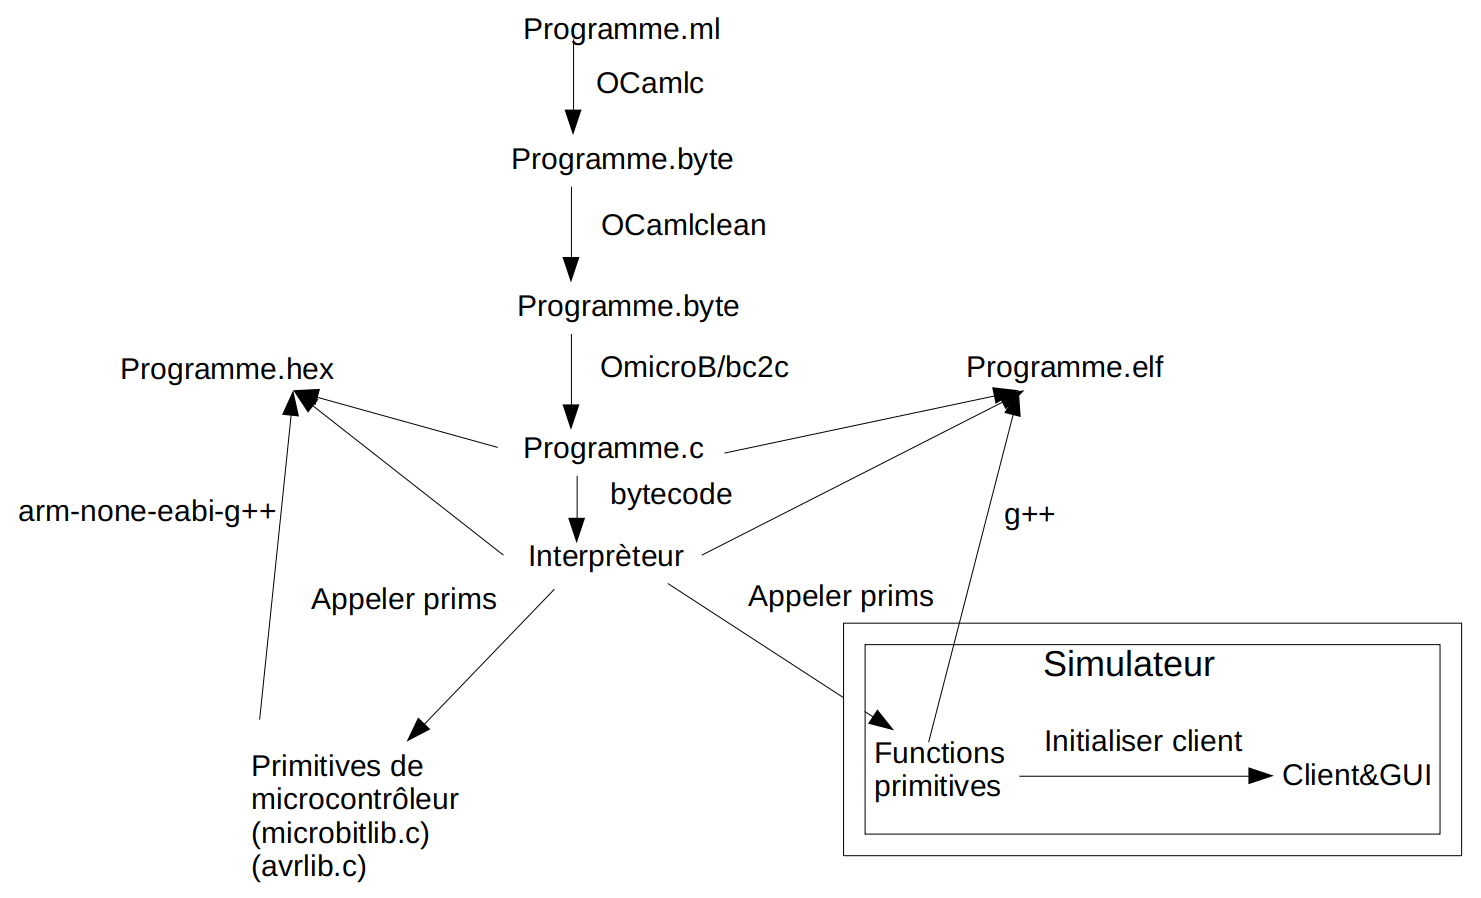
\includegraphics[width=\textwidth]{StructureProgramme.png}\\[1cm]
Cet image montre chaque étape de compilation d'un programme OCaml par OMicroB.
\begin{enumerate}
	\item \textbf{ocamlc} compile le fichier \textbf{.ml} avec la bibliothèque et génére un fichier \textbf{.byte}.
	\item \textbf{ocamlclean} traite le fichier généré \textbf{.byte}.
	\item \textbf{bc2c} est le compilateur de \textbf{OMicroB}, il permet de transférer le code binaire à un programme \textbf{.c}.
	\item \textbf{g++} compile le \textbf{programme.c} et la bibliothèque de simulateur \textbf{sf-regs} puis génère le fichier exécutable \textbf{.elf}.
	\item \textbf{arm-none-eabi-g++} compile le \textbf{programme.c} avec la bibliothèque de microcontrôleur (avrlib, microbitlib, etc) puis génére le fichier exécutable \textbf{.hex}.\\
\end{enumerate}

\textbf{OMicroB} produit deux fichiers exécutables après de compiler un programme \textbf{OCaml}.

- \textbf{.elf} est exécutable en mode simulation, il permet de démarrer le simulateur et montrer le changement des états de pin et les effets de programme sur une interface graphique.\\
- \textbf{.hex} est exécutable sur un microcontrôleur.

\clearpage
\pagestyle{fancy}
\lhead{Composition du simulateur}
\rhead{\thepage}
\fancyfoot{}
\section{Composition du simulateur}
Le simulatuer est composé du coté de client et du coté de serveur, ainsi que un langage de description pour le montage des périphériques sur un microcontrôleur.

\subsection{Montage}
Pour démarrer le processus client et implémenter l'interface graphique, le client a besoin de savoir quels composants du microcontrôleur il doit visualiser sur l'interface graphique. Donc 
nous devons proposer un fichier \textbf{circuit.txt} qui décrit les composants du microcontrôleur et les associations entre chaque composant et les pins correspondants. Avant de démarrer le processus client, le processus analyse est exécuté pour évaluer ce fichier. Une structure qui contient ces informations est stockée dans un mémoire partagé après l'évaluation. Le client peut recevoir les informations des composants du microcontrôleur depuis ce mémoire partagé.\\
Cette fonctionnalité est réalisée dans le dossier \textbf{src/byterun/montage}, la structure est définie dans \textbf{src/byterun/simul/share.h}.


\subsection{Client}
La partie client est programmée par C dans \textbf{src/byterun/client}, se compose de deux fichiers. 
\begin{enumerate}
\item \textbf{client.c} définit les fonctions du travail par exemple traiter le message qui vient du côté server.

\item \textbf{gui.c} implémente l'interface graphique par \textbf{gtk3.0}.
il nous montre un UI de simulateur permet de visualiser le résultat de programme et les états des pins pendant la simulation, ainsi que l'interaction par les boutons.\\
\end{enumerate}
 
\subsection{Serveur}
La partie serveur est codée par C dans "/src/byterun/", il contient des fichiers:
\begin{enumerate}
\item \textbf{/src/byterun/vm}. 
Ce dossier contient les fichiers de l'interprèteur d'OMicroB, par exemple le format des type basiques de données, le gc de machine virtuelle ainsi que les définition des instructions de code binaire. Il exécute le programme OCaml et envoie les instructions des codes binaires au serveur.

\item \textbf{/src/byterun/simul/sf-regs.c/.h}. 
C'est la bibliothèque des primitives de simulateur, lorsque le programme utilise un primitive par exemple \textbf{set\_pin}, l'interprèteur va appeler le primitive correspondant dans la bibliothèque, le serveur envoie l'instruction au côté client après le calcul.

\item \textbf{src/byterun/shared.c/.h}. 
Ce fichier définit des structures de données partagées
entre le processus client et serveur, elles sont stockées dans un mémoire partagé au fur et mesure de l'exécution de programme.
\end{enumerate}


\clearpage
\pagestyle{fancy}
\lhead{Mécanisme de communication}
\rhead{\thepage}
\fancyfoot{}
\section{Architecture du simulateur}
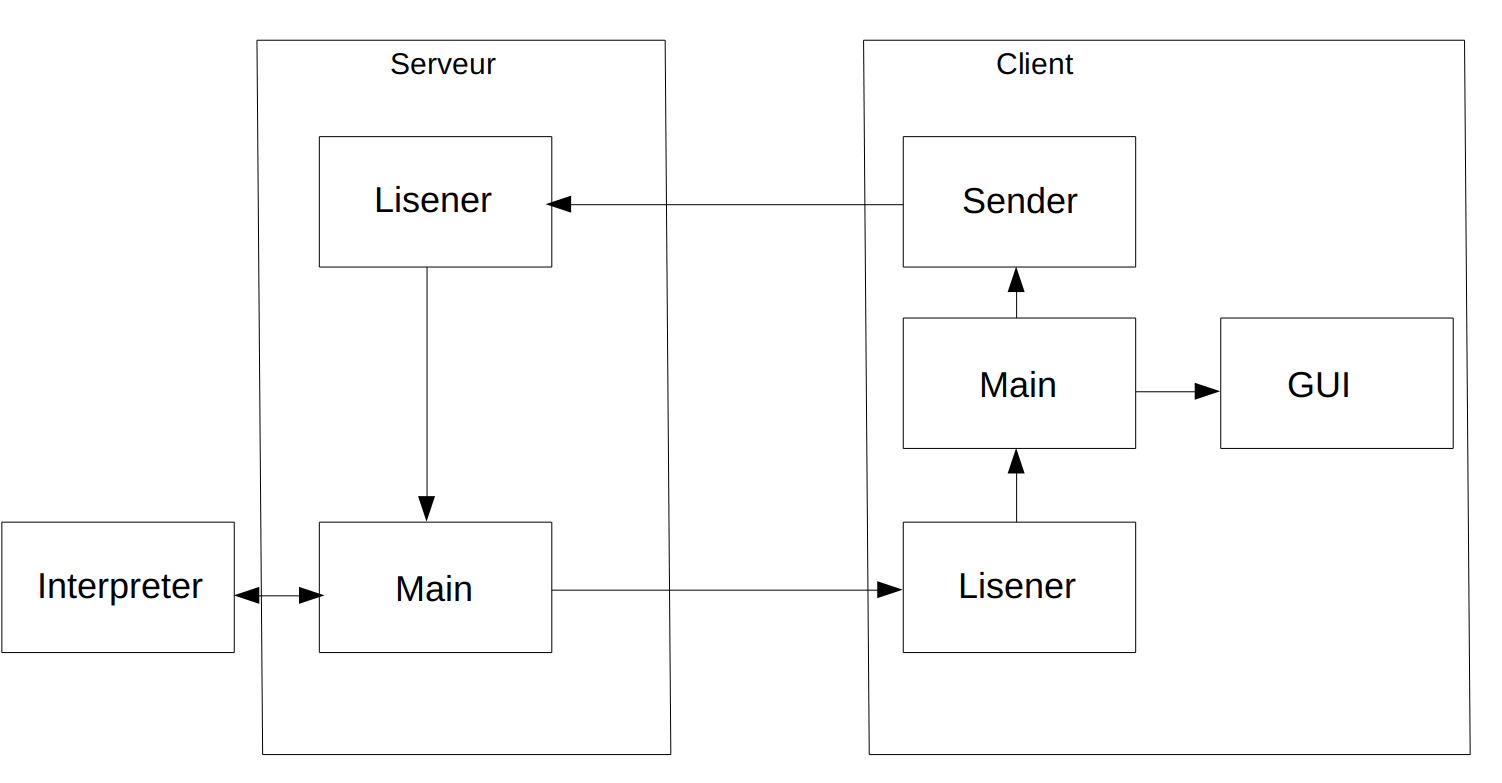
\includegraphics[width=\textwidth]{simulator.png}\\[1cm]
Cet image décrit globalement la structure du simulateur. On l'a réalisé par \textbf{l'architecture serveur-client} et il exécute deux processus en concurrence. Chaque processus exécute plusieurs threads et travaille asynchroniquement.\\

\textbf{Processus Serveur} exécute deux threads, \textbf{lisener} et \textbf{Main}.
\begin{enumerate}
	\item \textbf{Main} traite simplement l'instruction qui vient de l'interprèteur et envoyer au thread \textbf{lisener} de client.
	\item \textbf{lisener} reçoit l'instruction venant de \textbf{Sender} et informer \textbf{Main}.
\end{enumerate}

\textbf{Processus Client} tourne simultanément quatre threads, \textbf{Main}, \textbf{GUI}, \textbf{Sender} et \textbf{Lisener}.
\begin{enumerate}
	\item \textbf{Main} est le premier thread principal, il traite les arguments venant de processus serveur et connecte aux mémoires partagés, par exemple le mémoire partagé pour la communication et pour le montage. Il est responsable d'exécuter les autres threads.
	\item \textbf{GUI} crée les composants de l'interface graphique en fonction de l'information du montage. Il actualise l'interface dans un boucle infini afin de visualiser le changement des états de chaque composant simultanément.
	\item \textbf{Sender} sert à traiter input de l'utilisateur et envoyer l'instruction au serveur, par exemple appuyer les boutons. 
	\item \textbf{Lisener} reçoit l'instruction venant de serveur, en plus manipuler les composants de l'interface graphique en fonction de l'instruction.
\end{enumerate}

\subsection{Mécanisem de communication}
La mémoire partagée sert à communiquer entre le serveur et client, puisque c'est la plus rapide manière du transport de données. Mais son inconvénient est que l'on doit implémenter un mécanisme de synchronization afin de protéger les données partagées pour la lecture et l'écriture. Donc pour deux directions du transport (du serveur au client et du client au serveur), on a besoin de deux mémoires partagées, \textbf{shm1} est écrit par le serveur, le client le lit. \textbf{shm2} est inversé.\\

Afin de synchroniser la lecture et l'écriture, on met un mutex et une variable conditionnelle pour chaque mémoire partagée. Il garant que chaque instruction de serveur peut être bien traiter.

\textbf{Sénario de l'envoie une instruction}
\begin{enumerate}
	\item \textbf{client lisener} se bloque pour attendre l'instruction de serveur.
	\item \textbf{serveur main} demande le mutex
	\item \textbf{serveur main} vérifie la variable conditionnelle.\\
	- Si la condition se satisfait, il passe à l'étape suivant.
	- Sinon, cela veut dire que l'instruction dernière n'est pas encore traitée par client, \textbf{serveur main} se bloque.
	\item \textbf{serveur main} envoie l'instruction au client.
	\item \textbf{serveur main} débloque le thread \textbf{client lisener}.
	\item \textbf{serveur main} rend le mutex.
	\item \textbf{client lisener} est débloqué, demande le mutex.
	\item \textbf{client lisener} vérifie si la condition se satisfait.
	- Si oui, cela veut dire que la nouvelle instruction arrive, il passe à l'étape suivant.
	- Sinon, c'est un déblocage fausse, il se bloque.
	\item \textbf{client lisener} informe au \textbf{GUI} afin de visualiser le nouvel état de composant.
	\item \textbf{client lisener} débloque le thread \textbf{serveur main}.
	\item \textbf{client lisener} rend le mutex.
	\item retour à l'étape 1.
\end{enumerate}


\subsection{Protocode}
Protocode est un rôle de transfer les informations entre coté client et coté serveur.

0::25bits
~\\

(S -> C) Afficher un image représenté par 25bits sur l'écran.
~\\

1::x::y::val
~\\

(S -> C) Modifier l'état du pixel des coordonnées x et y à val.
~\\

2
~\\

(S -> C) Mettre les états de tous les pixels à 0
~\\

3::p::n
~\\

(S -> C) Modifier le pin p au niveau n. (n = 0 ou 1)
~\\

4::p::v
~\\

(S -> C) Modifier le pin p à la valeur v (0 <= v <= 1024).
~\\

0
~\\

(C -> S) Inverser l'état du bouton A.
~\\

1
~\\

(C -> S) Inverser l'état du bouton B.
~\\

Afin de représenter le protocol en un entier de 32 bits. on a utilisé 7bits pour le nom de fonction, alors on peut étendre jusqu'à 128 fonctions.
~\\

0::25bits
~\\

On juste lit 25 fois l'état de bit à partir de 8ieme bit. Pour modifier les états de pixel 0 au pixel 25. Mais cette commande n'est pas très extensible. Par exemple s'il y a plus pixel comme 10x10, alors on ne peut pas les représenter. Donc je veux plutôt réaliser cette fonction par setpixel. Cela veut dire que l'on appel le nombre de pixel fois setpixel pour afficher un image.
~\\

1::x::y::val. Cela veut dire écran[x][y]=val.
 x est représenté par 12bits, y aussi.
val est l'état de pixel, soit 0 soit 1 donc 1 bit est suffisant.  Donc la structure est 7::12::12::1=32bits
~\\

3::pin::niveau. Pin est représenté en 8bits,  niveau est 1 bit. La structure est 7::8::1=16bits
~\\


4::pin::valeur. Pin est aussi représenter en 8bits. Valeur est 17bits. Donc sa structure est 7::8::17=32
~\\

La différence entre 3 et 4 est que

la commande 3 est envoyé par la fonction microbit\_digital\_write qui permet de mettre le niveau de pin soit 0 soit 1.
la commande 4 est envoyé par microbit\_analog\_write qui peut modifier la valeur de pin. (0<=valeur<=1024)


\section{Fonctionalités Implémentées}
\subsection{Afficher les phrases à l'écran du simulateur}
Nous convertissons les informations de caractère dans la table Ascii en code hexadécimal 5x8 bits et les stockons dans un tableau, puis calculons le code ascii de chaque caractère un par un en recherchant. Utilisez-le pour calculer le décalage de ce caractère dans le tableau. Sortir enfin les 5 * 8 bits d'information dont il dispose. Prendre 5 * 5 bits d'entre eux et les imprimer pixel par pixel sur l'écran.
~\\

'A'

->

Ascii code =65

 ->

\{30,28,38,28,28\}

->

00110000

00101000

00111000

00101000

00101000

->

  **

  * *

  ***

  * *

  * *

\section{Sénarios et Tests}

\section{Difficulités Rencontrées}

Dans le processus de développement du programme, nous avons essayé diverses méthodes pour réaliser le transfert d'informations entre le client et le serveur. Au début, nous utilisions le pipe mais il était limité par la conception du programme. Le pipe n'avait aucun moyen de synchroniser le processus en fonctionnement. Plus tard, nous avons utilisé la méthode du signal pour transmettre des informations. Mais nous avons également constaté que parce qu'une action nécessite un signal défini par l'utilisateur pour être implémentée. Cependant, sur le système mac OS, il n'y a que deux signaux personnalisés que les utilisateurs peuvent utiliser. Nous avons donc également abandonné ce plan. Après de nombreuses tentatives, nous avons utilisé la méthode de la mémoire partagée et utilisé la variable mutex et de condiction pour synchroniser les processus.

\section{Conclusion}


\end{document}
